% This must be in the first 5 lines to tell arXiv to use pdfLaTeX, which is strongly recommended.
\pdfoutput=1
% In particular, the hyperref package requires pdfLaTeX in order to break URLs across lines.

\documentclass[11pt]{article}

% Remove the "review" option to generate the final version.
\usepackage[]{ACL2023}

% Standard package includes
\usepackage{times}
\usepackage{latexsym}

% For proper rendering and hyphenation of words containing Latin characters (including in bib files)
\usepackage[T1]{fontenc}
% For Vietnamese characters
% \usepackage[T5]{fontenc}
% See https://www.latex-project.org/help/documentation/encguide.pdf for other character sets

% This assumes your files are encoded as UTF8
\usepackage[utf8]{inputenc}

% This is not strictly necessary, and may be commented out.
% However, it will improve the layout of the manuscript,
% and will typically save some space.
\usepackage{microtype}

% This is also not strictly necessary, and may be commented out.
% However, it will improve the aesthetics of text in
% the typewriter font.
\usepackage{inconsolata}

\usepackage{booktabs} % for horizontal rules in tables
\usepackage{tabularx} % for tables with flexible width columns
\usepackage{graphicx}
\usepackage{subcaption}
\usepackage{amsmath}

\newcommand{\ap}[1]{{\color{red} AP: #1}}

% If the title and author information does not fit in the area allocated, uncomment the following
%
%\setlength\titlebox{<dim>}
%
% and set <dim> to something 5cm or larger.

\title{Rule-based Closed-loop Communication Detection}

% Author information can be set in various styles:
% For several authors from the same institution:
% \author{Author 1 \and ... \and Author n \\
%         Address line \\ ... \\ Address line}
% if the names do not fit well on one line use
%         Author 1 \\ {\bf Author 2} \\ ... \\ {\bf Author n} \\
% For authors from different institutions:
% \author{Author 1 \\ Address line \\  ... \\ Address line
%         \And  ... \And
%         Author n \\ Address line \\ ... \\ Address line}
% To start a seperate ``row'' of authors use \AND, as in
% \author{Author 1 \\ Address line \\  ... \\ Address line
%         \AND
%         Author 2 \\ Address line \\ ... \\ Address line \And
%         Author 3 \\ Address line \\ ... \\ Address line}

\author{Yuwei Wang \\
  University of Arizona \\
  \texttt{wangyw@arizona.edu}}

\begin{document}
\maketitle
\begin{abstract}
Closed-loop communication (CLC) is often recommended in the team research literature as a communication behavior that can secure the accuracy of information exchange, but detecting it in real-time presents a challenge as current methods rely on manual transcription and annotation. Current real-time dialog understanding or detection studies are limited to single human-computer interactions or pair-wise conversation detection, while CLC involves multiple turns and participants. To address this gap, this paper proposes a rule-based model that can detect CLC in spoken dialog within teams collaborating on shared tasks. Specifically, the paper proposes an algorithm for detecting the presence and breakdowns of CLC as they occur, with the ability to handle multiple participants. The proposed algorithm has the potential to be implemented in a real-time dialog event detection system.
\end{abstract}

\section{Introduction}

Effective teamwork is essential for achieving exceptional performance, particularly in complex or high-stakes settings and closed-loop communication (CLC) has been identified as a critical mechanism for successful teamwork \citep{salas2005there}. CLC refers to a communication practice in which feedback is provided to the sender to ensure that the message has been correctly received and understood, usually finalized by a final confirmation from the sender. While CLC has been demonstrated to improve team outcomes in various domains \citep{hargestam2016trauma, abd2018closed, bostrom2020mind}, detecting CLC in spoken dialog currently relies on retrospective analyses involving manual transcription and annotation. However, this approach is impractical in real-time settings where poor team communication can have catastrophic consequences. Thus, there is a pressing need for AI technologies that can detect and repair breakdowns in CLC as they occur. However, current dialog systems that understand and respond to human speech in real-time are typically limited to conversing with a single individual at a time. Furthermore, CLC often involves multiple turns of conversation and multiple participants, making pair-wise detection algorithms infeasible. To address this gap, this paper proposes building a CLC detection feature for an existing dialog system that can handle more general contexts, particularly those involving multiple participants. Specifically, this paper proposes a rule-based algorithm that can automatically detect the presence or absence of CLC and whether the loop has been closed in spoken dialog within teams of humans collaborating on shared tasks.

\subsection{Definition of CLC}
While different definitions of CLC can be found in the literature \citep{marzuki2019closed, hargestam2016trauma, abd2018closed, bostrom2020mind}, most of them involve a sequence of event phases, including call-out, check-back, and closing-of-the-loop. In the call-out phase, a speaker provides information or gives an instruction to another team member. In the following check-back event, the listener confirms their understanding of the information or instruction by repeating it back to the speaker. Finally, in closing-of-the-loop, the speaker confirms that the listener has received and understood the information or performed the desired action. 

\subsection{Previous Work}
Closed-loop communication (CLC) has been identified as an important component of effective team communication and has applications across different domains, such as medical emergencies, trauma team training, and highly regulated communications. 

\citet{hargestam2016trauma} conducted a study on communication in interdisciplinary teams, specifically exploring CLC during in situ trauma team training. The results showed that the use of CLC in trauma teams was limited, with an average of 20 closed-loop messages and 2.8 closed-loop communications per team. \citet{abd2018closed} have shown the ability of CLC to improve time-to-task completion in pediatric trauma activations. Their results showed that trauma activation with CLC was completed 3.6 times faster than those with open-loop communications. On the other hand, \citet{bostrom2020mind} investigated the use of closed-loop communication during icebreaker operations and whether it deviates from stipulated communication protocols. The study found that closed-loop communication practices inevitably incur feedback communication latency, leading to a tradeoff between high reliability and low latency.

Researchers have been using rule-based detection of dialog events for a long time because of its advantages over machine learning-based approaches in domain-specific tasks. The rule-based approach allows for rapid adaptation to changes in the experimental setup, structured events with complex structures, and transparency in the system's decisions, which facilitates maintainability and domain knowledge injection. Additionally, rule-based systems are easily modifiable, and their decisions can be immediately inspected \citep{nitschke2022rule}. The Odin event extraction framework is a state-of-art rule-based approach for  event extraction \citep{valenzuela-escarcega-etal-2016-odins}. It applies rules to identify events in natural language and has been used in the ASIST experiments \footnote{https://artificialsocialintelligence.org}, which simulates an urban search and rescue mission in Minecraft. \citet{nitschke2022rule} applied the Odin extraction framework to the ASIST experiment and achieved an F1 score of 0.77 for extracting complex events.

\section{Approach}
\subsection{The existing ToMCAT dialog system}
This project is built upon the existing ToMCAT dialog system \footnote{https://ml4ai.github.io/tomcat/}, including modules for automatic speech recognition (ASR) and event extraction. The current ToMCAT system can analyze spoken conversations in real-time, extract entities and events with a rule-based framework, and classify dialog acts and sentiments. As a goal, the proposed algorithm will enable the ToMCAT system to detect and repair breakdowns in CLC as they happen, thus enhancing its ability to support effective teamwork. 
\subsection{Odin}
The algorithm proposed in this study is built on the basis of event labels that are extracted by the Odin rules. Odin is a rule-based event extraction (EE) framework that consists of a declarative rule language and a runtime system for applying the rules. It extracts two broad types of events from natural language: simple events that do not have arguments, and complex events that can take other events as arguments. Each event is associated with a unique span of text and is assigned a label by the rule that extracts it. The event labels are organized into a hierarchical ontology, and if a rule assigns a label to an event, the parents of that label in the ontology are also assigned as labels for that event. The version of the ToMCAT dialog System used for this project and domain contains 420 active rules that map to a total of 238 event labels, including both parent labels and labels for targeted events. 

\subsection{The MultiCAT dataset}
To ensure adherence to information and data ethics, the CLC detection algorithm in this study was trained and evaluated using the MultiCAT dataset \citep{Culnan.ea:2023}. The dataset follows ethical requirements, including IRB protection for data and a data collection and process procedure that upholds ethical standards. The MultiCAT dataset was specifically designed for studying team collaboration in a search and rescue mission. In each trial of the study, a team of three participants conducted simulated urban search and rescue missions in a Minecraft-based virtual testbed with unique capabilities and information, aiming to maximize their score by completing the mission objectives within a 15-minute time limit. Participants' speech was recorded on separate channels and transcribed in real-time using Google's Cloud Speech-to-Text API. Researchers annotated a subset of the data for various features including CLC events, which were annotated jointly by one graduate student and the author.

The CLC annotation in the MultiCAT dataset adapted the MRDA (Multi-Dimensional Annotation) framework for annotating adjacency pairs and provides annotations for each CLC phase alongside the index for each CLC event, which enables us to precisely locate each CLC event especially when the check-back and closing-of-the-loop are several utterances away from the call-out.

The dataset contains 4929 utterances and was annotated with two types of labels for each utterance in a CLC event. These labels include the corresponding CLC components, as defined previously, and their communicative functions, following the work of \citet{marzuki2019closed} with some modifications. The dataset consists of 35 trials. There are 3227 instances of \textit{a}, 1993 instances of \textit{b}, and 431 instances of \textit{c}. Table  \ref{tab:clc-label-category} provides a summary of the CLC labels in the dataset. Table \ref{tab:clc-annotation-example} presents the component labels along with examples. In the dataset, it is common for a single utterance to be assigned multiple CLC labels as the first and the third utterances shown in the table.

CLC events span multiple utterances and involve coherent communication flows. Randomly selecting and splitting utterances into training and testing datasets would result in fragmented data, losing crucial relationships and contextual information within conversations. In our dataset, we have 32 trials, and within each trial, speakers maintain a continuous flow of conversation. To preserve the integrity of these conversations, I decided to randomly split the trials into a 70\% training dataset (rounding up to 22 trials) and a 30\% testing dataset (rounding down to 9 trials). This ensures that the training and testing data maintain the coherence and continuity necessary for accurate analysis of CLC events.

\begin{table}
    \centering
    \footnotesize
    \begin{tabularx}{\linewidth}{cX}
    \toprule
    Component & Communicative functions \\
    \midrule
       \texttt{a} & assert, action-directive, info-request, commit \\
       \texttt{b} & accept, reject, acknowledge, info-provide, follow-up-question \\
       \texttt{c} & accept, acknowledge, info-provide \\
       \bottomrule
    \end{tabularx}
    \caption{%
        CLC label categories in MultiCAT.
        The dataset uses \texttt{a} and \texttt{b} to annotate call-outs and checkbacks respectively and \texttt{c} for closings. Each component label has a set of possible communicative function labels that it can be paired with. 
    }
    \label{tab:clc-label-category}
\end{table}

\begin{table}
    \centering
    \footnotesize
    \begin{tabularx}{\linewidth}{p{0.8cm}XcX}
    \toprule
     Speaker & Utterance &  Label & Function\\
     \midrule
     BLUE & \emph{Okay I'm heading this way this is the engineer which room did you say you needed help with}    & 72a.73a & assert.info-request\\
     GREEN & \emph{follow green it is E3 yes so both} & 73b & info-provide\\
     BLUE & \emph{all right E3 okay I lost green green Green is too fast} & 73c.74a & acknowledge.assert\\
     \bottomrule
    \end{tabularx}
    \caption{Examples of annotations in the dataset. The ``Label'' column labels CLC phases and their indices indicating the Nth adjacency pairs in the current trial following the MRDA framework. The ``Function'' column indicates the communicative function of the utterance.}
    \label{tab:clc-annotation-example}
\end{table}

\subsection{Model development procedure}
To ensure a systematic development process, I divided the model development into two steps. Firstly, I selected a suitable set of event labels that correspond to each stage of CLC. Subsequently, I designed and implemented an algorithm capable of accurately identifying these phases within a conversation. To enhance performance, I engaged in iterative evaluation and development for both steps.

\subsection{Model performance evaluation}
In this study, the performance of the event extraction model is assessed using commonly used metrics in natural language processing, namely accuracy, precision, recall, and F1 score. These metrics collectively provide a comprehensive analysis of the model's performance.

I conducted two evaluations to assess the performance of our CLC event detection system. The first evaluation followed a strict form, considering the complete CLC event. To capture different degrees of closure in the communication process, we also conducted a slightly more relaxed evaluation. The results from these evaluations provide insights into the performance of our system in detecting both strict and relaxed closed-loop communication instances.

\section{Model}
The model development process consists of two steps: selecting appropriate event labels for each stage of CLC, and then creating an algorithm to accurately detect these phases in conversations.

\subsection{Label selection}
Selecting appropriate event label sets for each CLC phase is a crucial step before detecting CLC events in conversation because the event labels serve as identifiers to categorize different phases within a conversation. This ensures that the algorithm can accurately recognize and differentiate between these stages.

To select labels for each phase of CLC, I match the CLC phase annotation with event labels extracted using the Odin rule of the ToMCAT dialog System. For example, in the call-out phase \textit{a}, I create a frequency table of associated event labels to gain an overview of their representations. I iteratively consider the Nth most frequent set of event labels, ranging from most to least frequent, to evaluate detection metrics (accuracy, precision, recall, and F1) and determine the optimal balance. The selected label set achieving this balance becomes the designated label set for the phase \textit{a}. This process is repeated for each CLC stage to establish appropriate event label selections. 

Figure \ref{fig:label_selection} depicts the detection metrics for the three CLC phases, highlighting the relationship between accuracy and recall. The call-out stage shows a positive correlation between these metrics, exhibiting consistent growth until approximately the selection of the first 25 frequent labels. Conversely, the check-back and closing-of-the-loop stages demonstrate a negative correlation. To strike a balance between accuracy and recall, the intersection point where these metrics converge serves as a suitable decision criterion for label set selection. The observed pattern aligns with the nature of each phase, where the call-out stage encompasses various event types such as questions, requests, instructions, assertions, and commitments, while the check-back and closing-of-the-loop stages involve more repetitive events like acknowledgment, acceptance, or knowledge sharing. Based on these observations, the 25 most frequent event labels for call-out, 4 most frequent labels for check-back, and 2 most frequent labels for closing-of-the-loop are selected as the labels for CLC event detection. Appendix \ref{appendix:label_selection} provides a list of the selected event labels for each CLC phase.

\captionsetup[subfigure]{width=1.25\textwidth}
\begin{figure}
  \centering
  \begin{subfigure}{0.32\textwidth}
    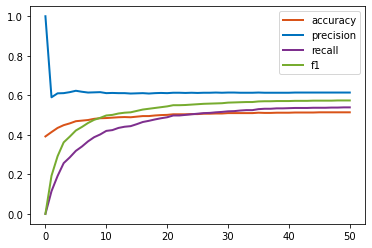
\includegraphics[width=\linewidth]{callout.png}
    \caption{Label Selection Metrics for Call-out}
    \label{fig:plot1}
  \end{subfigure}
  \hfill
  \begin{subfigure}{0.32\textwidth}
    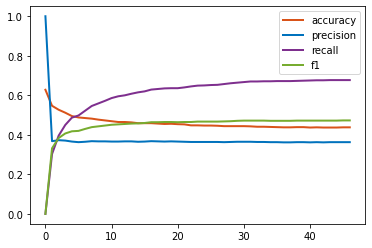
\includegraphics[width=\linewidth]{checkback.png}
    \caption{Label Selection Metrics for Check-back}
    \label{fig:plot2}
  \end{subfigure}
  \hfill
  \begin{subfigure}{0.32\textwidth}
    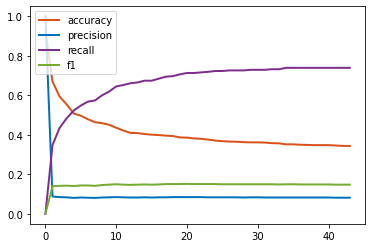
\includegraphics[width=\linewidth]{closing.png}
    \caption{Label Selection Metrics for Closing-of-the-loop}
    \label{fig:plot3}
  \end{subfigure}

  \caption{Metrics for event label selection based on frequency. The x-axis represents the number of selected labels from the event label frequency table, where 1 corresponds to the most frequently occurring single event label, and N corresponds to the Nth most frequent set of event labels.}
  \label{fig:label_selection}
\end{figure}

\subsection{Pattern recognition}
The CLC pattern detection process begins by identifying call-outs in each utterance of the corpus. If an utterance contains any event label from the selected call-out label set, it is labeled as phase \textit{a}. Subsequently, the analysis extends to the following utterances within a specified window size to identify check-backs or closing-of-the-loop events. If such events are detected, the "a" label is augmented with additional \textit{b} or \textit{c} labels accordingly, reflecting the presence of check-backs or closing-of-the-loop phases for the current utterance. Conversely, if an utterance is not a call-out, it is assigned the \textit{NA} label to indicate that it does not mark the beginning of a CLC event. The \textit{window\_size} parameter allows flexibility in determining the range of subsequent utterances considered following the current utterance. Through this procedure, CLC patterns can be effectively identified and labeled throughout the corpus.

\section{Result}
The CLC event detection is assessed by iterating through different window sizes ranging from 3 to 10. Notably, as the window size increases, the accuracy exhibits a decreasing trend. This observation suggests that larger window sizes may lead to potential overfitting of the model. Table \ref{tab:clc_results} presents the overall evaluation metrics for the CLC event detection with a specific window size of 3. Since each utterance is assigned a CLC event label from one of the four categories (i.e. \textit{NA}, \textit{a}, \textit{ab}, and \textit{abc}), the evaluation can be likened to a classification task with four classes.

\begin{table}[h]
    \centering
    \begin{tabularx}{\linewidth}{p{0.7cm}cccc}
        \toprule
        Label & Precision & Recall & F1 & Support \\
        \midrule
        NA   & 0.662   & 0.695   & 0.678   & 800 \\
        a    & 0.340   & 0.382   & 0.360   & 374 \\
        ab   & 0.275   & 0.261   & 0.268   & 272 \\
        abc  & 0.000   & 0.000   & 0.000   & 74 \\
        \bottomrule
        Accuracy & \multicolumn{4}{c}{0.507} \\
        \bottomrule
    \end{tabularx}
    \caption{Results for Strict CLC Event Detection}
    \label{tab:clc_results}
\end{table}

\begin{table}[h]
    \centering
    \begin{tabularx}{\linewidth}{p{0.7cm}cccc}
        \toprule
        Label & Precision & Recall & F1 & Support \\
        \midrule
        NA      & 0.662   & 0.695   & 0.678   & 800 \\
        closed  & 0.340   & 0.254   & 0.291   & 346 \\
        open    & 0.340   & 0.382   & 0.360   & 374 \\
        \bottomrule
        Accuracy & \multicolumn{4}{c}{0.518} \\
        \bottomrule
    \end{tabularx}
    \caption{Results for Relaxed CLC Event Detection}
    \label{tab:clc_relaxed_results}
\end{table}


Upon analyzing the resulting scores, we observe that the overall accuracy score for the four classes is slightly above 50\%. In the context of a four-class classification problem, the naive guess for overall accuracy would be to randomly assign each instance to one of the four classes. Assuming a balanced dataset, this random guess would yield an overall accuracy of approximately 25\%. Therefore, the achieved accuracy of over 50\% indicates a significant improvement compared to random guessing.

However, it is important to note that the accuracy is significantly influenced by the \textit{NA} category, which exhibits an F1 score of 0.677. This category also has the highest support, indicating an imbalance in the distribution of labels across the classes.

Among the CLC event categories, the next best performance is observed in call-out detection, which represents the initial stage of open-loop communication. The \textit{ab} category follows with comparatively lower performance, while the full completion CLC event detection achieves an F1 score of 0.

I observed that the complete form of the CLC event is relatively rare in our dataset (279 out of 4929), which is consistent with findings reported by other researchers \citep{hargestam2016trauma, marzuki2019closed}. To evaluate whether the communication loop is completely open or partially closed, I conducted a slightly relaxed version of the evaluation. If an utterance is labeled only with \textit{a}, it is marked as open-loop communication. On the other hand, if an utterance is labeled with \textit{ab} or \textit{abc}, it is considered relaxed closed-loop communication. This approach allows us to capture different degrees of closure in the communication process. The results of this additional evaluation are presented in Table \ref{tab:clc_relaxed_results}. Notably, the overall accuracy shows a slight increase, and the detection of the relaxed closing form of the CLC event yields significantly better metrics compared to the complete closing form of CLC evaluation (i.e. the \textit{abc} form).

\section{Discussion}

The rule-based model presented in this study offers several highlights in the context of CLC event detection. Firstly, the utilization of predefined event labels enables us to perform a comprehensive evaluation of the algorithm's performance against ground truth annotations or human-labeled data. This evaluation allows us to quantify the accuracy, precision, recall, and other pertinent metrics, providing valuable insights into the effectiveness of the algorithm in detecting CLC events. By comparing the algorithm's output with the ground truth, we can assess its ability to accurately capture and classify the various stages and sub-stages of CLC.

Furthermore, the rule-based model exhibits a high degree of customization and adaptability. Recognizing that different domains or applications may involve variations in the stages or sub-stages of CLC, the model allows for the selection of appropriate event labels. This customization process empowers us to tailor the detection algorithm to the specific requirements and variations of the target domain. By adapting the model to the unique characteristics of the domain, we enhance its versatility and effectiveness in detecting CLC events. This flexibility is particularly valuable as it enables the model to be applied to a wide range of communication scenarios, ensuring its applicability across diverse contexts.

Despite the strengths of the study, there are certain weaknesses that need to be acknowledged. Firstly, the scarcity of training data for sparse labels such as the \textit{abc} sequence event poses a challenge to the detection of the complete form of CLC events. Additionally, the high frequency of event labels associated with the closing-of-the-loop stage may have introduced potential issues related to overfitting, as the model becomes more inclined to favor these commonly occurring labels at the expense of detecting rarer or more nuanced patterns. These challenges highlight the need for a larger and more diverse dataset that adequately represents the full range of CLC event variations.

Another weakness stems from the nature of rule-based label selection, which inherently involves a trade-off between precision and recall. The process of defining rules and selecting event labels based on specific criteria can result in certain events being either missed or incorrectly classified. This trade-off can affect the overall accuracy and performance of the model, particularly in situations where there are ambiguous or overlapping event patterns.

To address these weaknesses and improve the performance of the model, several future improvements can be considered. Firstly, increasing the availability of training data for sparse labels, such as the \textit{abc} sequence event, would provide the model with more examples to learn from, enabling better detection and classification. Additionally, carefully selecting combinations of event labels and refining the rules used in the label selection process can contribute to enhancing the precision, recall, and overall accuracy of the model. By continuously refining and updating the rule-based approach, the model can adapt to the complexities and variations present in different communication contexts.

\section{Conclusion}
This study presents a rule-based model for detecting CLC events in conversations. The model utilizes event labels generated by the ToMCAT dialog agent and selects label sets to represent each phase of the CLC events. Evaluation results show an overall accuracy of 0.505 for strict CLC event detection and an accuracy of 0.521 for a relaxed CLC form. The rule-based model demonstrates its effectiveness by outperforming chance by approximately 25\%.

The model's adaptability allows for seamless integration into different domains and applications, enabling customized CLC event detection based on specific requirements and variations. However, limitations are identified, including the scarcity of training data for sparse labels like the \textit{abc} sequence event and the inherent trade-off between precision and recall in the label selection process.

Future research should address these weaknesses and further enhance the rule-based model. Improvements can be made by carefully selecting combinations of event labels that align with the communication domain's characteristics. Additionally, expanding the training dataset to encompass a broader range of CLC events and variations would mitigate limitations associated with sparse labels.

In conclusion, while the rule-based model demonstrates strengths in evaluating and customizing CLC event detection, ongoing research is needed to overcome weaknesses and fully harness its potential in analyzing and understanding CLC events in diverse communication contexts.

\section*{Github Repo}
\href{https://github.com/Yuweien/INFO699-clc-detection.git}{https://github.com/Yuweien/INFO699-clc-detection.git}

% Entries for the entire Anthology, followed by custom entries
\bibliography{anthology,custom}
\bibliographystyle{acl_natbib}

\appendix

\section{Example Appendix}
\label{appendix:label_selection}

\begin{itemize}
  \item \textbf{Event label selection for the call-out phase}
    KnowledgeSharing
    
    DeliberatePlan
    
    YesNoQuestion
    
    Precedence
    
    MoveTo
    
    MakeCommitment
    
    Instruction
    
    ReportLocation
    
    Gratitude
    
    OnMyWay
    
    ContingentPlan
    
    Question
    
    NeedAction
    
    Search
    
    NeedPresence
    
    LocationQuestion
    
    Block
    
    MarkerBlock
    
    Meeting
    
    Disagreement
    
    AmTrapped
    
    HelpRequest
    
    TimeUnit
    
    Enter
  \item \textbf{Event label selection for the check-back phase}

    Agreement

    KnowledgeSharing
    
    YesNoQuestion
    
    DeliberatePlan

  \item \textbf{Event label selection for the closing-of-the-loop phase}
  
    Agreement

    KnowledgeSharing
  
\end{itemize}





\end{document}
